%%%%%%%%%%%%%%%%%%%%%%%%%%%%%%%%%%%%%%%%%
% baposter Landscape Poster
% LaTeX Template
% Version 1.0 (11/06/13)
%
% baposter Class Created by:
% Brian Amberg (baposter@brian-amberg.de)
%
% This template has been downloaded from:
% http://www.LaTeXTemplates.com
%
% License:
% CC BY-NC-SA 3.0 (http://creativecommons.org/licenses/by-nc-sa/3.0/)
%
%%%%%%%%%%%%%%%%%%%%%%%%%%%%%%%%%%%%%%%%%

%----------------------------------------------------------------------------------------
%	PACKAGES AND OTHER DOCUMENT CONFIGURATIONS
%----------------------------------------------------------------------------------------

\PassOptionsToPackage{dvipsnames}{xcolor}
\documentclass[portratit,a1paper,fontscale=0.58]{baposter} % Adjust the font scale/size here 0.285

\usepackage{natbib}

%\usepackage[usenames]{color}
%\usepackage{colortbl}
%\usepackage[usenames,dvipsnames,svgnames,table]{xcolor}
\usepackage{wrapfig}

\usepackage{graphicx} % Required for including images
\graphicspath{{figures/}} % Directory in which figures are stored

\usepackage{amsmath} % For typesetting math
\usepackage{amssymb} % Adds new symbols to be used in math mode

\usepackage{booktabs} % Top and bottom rules for tables
\usepackage{enumitem} % Used to reduce itemize/enumerate spacing
\usepackage{palatino} % Use the Palatino font
\usepackage[font=small,labelfont=bf]{caption} % Required for specifying captions to tables and figures

\usepackage{multicol} % Required for multiple columns
\setlength{\columnsep}{1.5em} % Slightly increase the space between columns
\setlength{\columnseprule}{0mm} % No horizontal rule between columns

%\usepackage[T1]{fontenc}
%\usepackage{mathtools}
%\usepackage{empheq}
%\usepackage[dvipsnames]{xcolor}

\usepackage{tikz} % Required for flow chart
\usetikzlibrary{shapes,arrows} % Tikz libraries required for the flow chart in the template

\newcommand{\compresslist}{ % Define a command to reduce spacing within itemize/enumerate environments, this is used right after \begin{itemize} or \begin{enumerate}
\setlength{\itemsep}{1pt}
\setlength{\parskip}{0pt}
\setlength{\parsep}{0pt}
}

\definecolor{lightblue}{rgb}{0.145,0.6666,1} % Defines the color used for content box headers

%%%%%%%%%%%%%%%%%%%% User-defined commands %%%%%%%%%%%%%%%%%%%%%%%%

\newcommand{\la}{\langle}
\newcommand{\ra}{\rangle}

\newcommand{\ua}{\uparrow}
\newcommand{\da}{\downarrow}

\newcommand{\gs}{{\rm gs}}
\newcommand{\GS}{{\rm GS}}
\newcommand{\kF}{k_{\rm F}}

\newcommand{\mi}{ m}

\renewcommand{\H}{\hat H}

\newcommand{\Ptot}{\hat P_{\rm tot}}
\newcommand{\mfp}{\lambda_*}

\newcommand{\Htot}{\hat H}

\newcommand{\Hh}{\hat H_{\rm h}}
\newcommand{\Eh}{E_{\rm h}}

\newcommand{\Hi}{\hat H_{\rm i}}
\newcommand{\Ei}{E_{\rm i}}

\newcommand{\U}{\hat U}

\newcommand{\V}{\hat V}

\newcommand{\rr}{{\mathbf r}}

\newcommand{\vv}{{\mathbf v}}

\newcommand{\Vi}{{\mathbf {\hat V}_{\rm i}}}

\newcommand{\vGS}{v_{\mathsmaller{\rm GS}}}
\newcommand{\vvGS}{{\bf v}_{\mathsmaller{\rm GS}}}

\newcommand{\q}{{\mathbf q}}

\newcommand{\p}{{\mathbf p}}
\newcommand{\pp}{\hat {\mathbf P}}
\newcommand{\ppi}{\hat {\mathbf P}_{\rm imp}}
\newcommand{\pph}{\hat {\mathbf P}_{\rm h}}

\newcommand{\disp}{{\cal E}}

\newcommand{\be}{\begin{equation}}
\newcommand{\ee}{\end{equation}}

\newcommand{\bra}[1]{\left\langle{#1}\right|}
\newcommand{\ket}[1]{\left|{#1}\right\rangle}

\newcommand{\h}{\hbar}

\newcommand{\kB}{k_B}
\newcommand{\tr}{\mathop{tr}}
\newcommand{\sqs}{\mbox{\fbox{$\sigma$}}}

\newcommand{\ssigma}{{\boldsymbol{\sigma}}}
\newcommand{\cc}{{\boldsymbol{\sigma}}}

%%%%%%%%%%%%%%%%%%%%%%%%%%%%%%%%%%%%%%%%%%%%%%%%%%%%%%%%%%%%%%%%%%%%%

\begin{document}

\begin{poster}
{
headerborder=closed, % Adds a border around the header of content boxes
colspacing=1em, % Column spacing
bgColorOne=white, % Background color for the gradient on the left side of the poster
bgColorTwo=white, % Background color for the gradient on the right side of the poster
borderColor=lightblue, % Border color
headerColorOne=black, % Background color for the header in the content boxes (left side)
headerColorTwo=lightblue, % Background color for the header in the content boxes (right side)
headerFontColor=white, % Text color for the header text in the content boxes
boxColorOne=white, % Background color of the content boxes
textborder=roundedleft, % Format of the border around content boxes, can be: none, bars, coils, triangles, rectangle, rounded, roundedsmall, roundedright or faded
eyecatcher=true, % Set to false for ignoring the left logo in the title and move the title left
headerheight=0.1\textheight, % Height of the header
headershape=roundedright, % Specify the rounded corner in the content box headers, can be: rectangle, small-rounded, roundedright, roundedleft or rounded
headerfont=\Large\bf\textsc, % Large, bold and sans serif font in the headers of content boxes
%textfont={\setlength{\parindent}{1.5em}}, % Uncomment for paragraph indentation
linewidth=2pt, % Width of the border lines around content boxes
columns=2
}
%----------------------------------------------------------------------------------------
%	TITLE SECTION
%----------------------------------------------------------------------------------------
%
{
\includegraphics[height=4 em]{skoltech_logo.png}} % First university/lab logo on the left
{
\bf{\LARGE An algebraic approach to spin-1/2 systems with isotropic Heisenberg interaction}
\vspace{0.4em}
} % Poster title
{\textsc{ \large Filipp Uskov  \\
\vspace{5 pt}
\textcolor{blue}{Skoltech}    \hspace{12pt} \textcolor{blue}{Moscow State University}
 }\\
 \vspace{3 pt}
{\small in collaboration with Oleg Lychkovsky and Elena Shpagina}} % Author names and institution
{
\begin{tabular}{c}

\includegraphics[height=4.5 em]{msuLogo.png}
%\includegraphics[height=3 em]{logoRQC.png}
\end{tabular}
} % Second university/lab logo on the right



%----------------------------------------------------------------------------------------
%	Question
%----------------------------------------------------------------------------------------

\headerbox{Motivation}{name=motivation,column=0,row=0,span=1}
{
In many problems involving spin-1/2 systems with isotropic Heisenberg interaction one needs to simplify products of scalar and mixed products of Pauli matrices.

\vspace{0.5em}

Tipical hamiltonian: $H=\sum_{<i,j>}(\ssigma_i \ssigma_j)$

$<i,j>$ - denotes neighbours particles

\vspace{0.5em}

Typical problems of such systems:
\begin{itemize}
\item squaring parametrization [1]%\cite{sqparam}
\item variational principle [3]%\cite{TarrahValenti}
\item Schrodinger equation in the form $H\rho=E\rho$ [2]%\cite{hroero}
[see also poster by E. Spagina]
\end{itemize}

Important: account for all (possibly noncommuting) symmetries simultaneously!
}

%----------------------------------------------------------------------------------------

\headerbox{Contracted Shredinger equation}{name=shredinger,column=0,below=motivation,span=1}{
Equation $H\psi=E\psi$ is equal[2]  %\cite{hroero} 
to $H\rho=E\rho$, where $\rho$ is dansity matrix.

Then we seek $\rho$ in form accounting rotation, inverse time and hamiltonian simmetries: 
$$\frac{1}{2^N}(1+a_{i,j}(\ssigma_i \ssigma_j)+b_{i,j,k,l}(\ssigma_i \ssigma_j)(\ssigma_k \ssigma_l)+e.t.c.).$$

Scalar product on such matrices: $(A,B):=\tr(AB)$,

Ortonormal basis $1,(\ssigma_i \ssigma_j),\;(\ssigma_i \ssigma_j)(\ssigma_k \ssigma_l),\;e.t.c.$

\begin{center} \textcolor{green}{Example:} \end{center}
$$H=(\cc_1,\cc_2)+(\cc_2,\cc_3)$$ 
seek $\rho$ taking into account Hamiltonian symmetry $1\leftrightarrow 3$
$$\rho = \frac18(1+a((\cc_1,\cc_2)+(\cc_2,\cc_3))+b(\cc_1,\cc_3))$$

$$\begin{gathered}
H\rho=\frac18((\cc_1,\cc_2)+(\cc_2,\cc_3)) (1+a((\cc_1,\cc_2)+(\cc_2,\cc_3))+b(\cc_1,\cc_3)) =\\
= \frac18(6 a +(1+b- 2 a) (\cc_1, \cc_2)  + 2 a (\cc_1, \cc_3) +(1+b- 2 a) (\cc_2, \cc_3)) =\\
= \frac18(E+E a(\cc_1,\cc_2)+E a(\cc_2,\cc_3) + E b(\cc_1,\cc_3)) = E\rho
\end{gathered}$$

Then we get system of three different quadratiq equations:

$$
\begin{cases}
6 a-E=0\\
1-2 a+b-a E=0\\
2 a-b E=0
\end{cases}
$$

and then we solve it:

$$
\begin{cases}
a=-\frac12 \\b= \frac13 \\E=-4
\end{cases} \quad
\begin{cases}
a=0 \\b=-1 \\E=0
\end{cases} \quad
\begin{cases}
a=\frac13 \\b=\frac13 \\E=2
\end{cases} \quad
$$
}

%----------------------------------------------------------------------------------------

\headerbox{Variational Principle}{name=varpr,column=0,below=shredinger,span=1}{ 
According variational principle[3] wis $N$ spins ground state energy of all lattice
$$E_{gs}\geqslant\frac{2N}{M}\min_\rho\tr H\rho$$
where $H$ and $\rho$ -- for some cluster with $M$ interactions.

\begin{wrapfigure}{r}{0.2\textwidth}
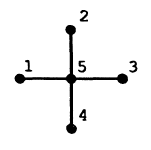
\includegraphics[width=0.2\textwidth]{cluster-crest.png}
\end{wrapfigure}

\vspace{0.5em}

\textcolor{green}{Example:} $H=(\cc_1,\cc_5)+(\cc_2,\cc_5)+(\cc_3,\cc_5)+(\cc_4,\cc_5)$

%image

$\rho$ should be positive semidefinite, so we parametrize[1] it by $\tau$: $\rho=\frac{\tau^2}{\tr\tau^2}$

According to lattice simmetries we seek
$$\begin{gathered}
\tau=1 + \\
a_1 ((\cc_1, \cc_5) + (\cc_2, \cc_5) + (\cc_3, \cc_5) + (\cc_4, \cc_5)) + \\
a_2 ((\cc_1, \cc_3) + (\cc_2, \cc_4)) + \\
a_3 ((\cc_1, \cc_2) + (\cc_2, \cc_3) + (\cc_3, \cc_4) + (\cc_4, \cc_1)) + \\
b_1 ((\cc_1, \cc_5) (\cc_2, \cc_3) + (\cc_1, \cc_5) (\cc_4, \cc_3) + (\cc_2, \cc_5) (\cc_3, \cc_4) + (\cc_2, \cc_5) (\cc_1, \cc_4) + \\
+ (\cc_3, \cc_5) (\cc_4, \cc_1) + (\cc_3, \cc_5) (\cc_2, \cc_1) + (\cc_4, \cc_5) (\cc_1, \cc_2) + (\cc_4, \cc_5) (\cc_3, \cc_2)) + \\
b_2 ((\cc_1, \cc_2) (\cc_3, \cc_4) + (\cc_2, \cc_3) (\cc_4, \cc_1)) + \\
b_3 (\cc_1, \cc_3) (\cc_2, \cc_4) + \\
b_4 ((\cc_1, \cc_5) (\cc_2, \cc_4) + (\cc_2, \cc_5) (\cc_1, \cc_3) + (\cc_3, \cc_5) (\cc_2, \cc_4) + (\cc_4, \cc_5) (\cc_1, \cc_3))
\end{gathered}$$

$$\tr H\rho = \frac{\begin{gathered}(
24 a_1 - 24 a_1^2 + 24 a_1 a_2 + 48 a_1 a_3 + 48 a_2 b_1 + 192 a_3 b_1 - 192 b_1^2 + 192 b_1 b_2 + \\
48 b_1 b_3 + 72 a_2 b_4 + 48 a_3 b_4 - 96 b_1 b_4 + 48 b_2 b_4 + 72 b_3 b_4 - 72 b_4^2)\end{gathered}}
{1 + 12 a_1^2 + 6 a_2^2 + 12 a_3^2 + 96 b_1^2 + 24 b_2^2 + 12 b_2 b_3 + 9 b_3^2 + 48 b_1 b_4 + 36 b_4^2}$$

$$NMinimize\rightarrow\Bigg\{-6., \begin{cases}
a_1 \rightarrow -0.5,&a_2 \rightarrow 0.333333, \\a_3 \rightarrow 0.333333, \\
b_1 \rightarrow -0.1,&b_2 \rightarrow 0.0666667,\\
b_3 \rightarrow 0.0666667, &b_4 \rightarrow -0.1
\end{cases}\Bigg\} \quad\Rightarrow\quad
E_{gs}\geqslant\frac{2N}{4}(-6)
$$

The same result was obtained by another method in [4]

We expect that our method outperforms the method of ref. [4] for larger clusters.

\textcolor{red}{Work is underway.}
}

%----------------------------------------------------------------------------------------
%----------------------------------------------------------------------------------------

\headerbox{Algorithm for simplification $\sigma$-matrices}{name=sigmaalg,column=1,row=0,span=1}{ %symbolic
This algorithm used for multiplication $H\rho$ and other multiplications.

\vspace{0.5em}
%\hline(1,0){20em}
$\rightarrow$ 
Input and output form: $(\ssigma_i \ssigma_j) = d(i,j)$ and $(\ssigma_i \ssigma_j \ssigma_k) = t(i,j,k)$.

Algorithm:
\begin{enumerate}
	\item 
	\begin{itemize}
		\item $d(i,j)\rightarrow\sigma(i,\alpha)\sigma(j,\alpha)$
		\item $t(i,j,k)\rightarrow\varepsilon(\alpha,\beta,\gamma)\sigma(i,\alpha)\sigma(j,\beta)\sigma(k,\gamma)$
	\end{itemize}
	\textcolor{Gray}{(we assume that different spin indices are different: $i\neq j\neq k\neq i$ etc)}

	\item \textcolor{Gray}{$\sigma$-matrices with different spin indices are commuting, so we can} stable(!) sort it:
	\begin{enumerate}
		\item first $\sigma$ in multiplication $\rightarrow \tilde\sigma$
		\item while found $\tilde\sigma\sigma$
		\begin{enumerate}
			\item $\tilde\sigma\sigma \rightarrow \tilde\sigma\sqs$
			\item while found $\tilde\sigma\sqs$
			\begin{enumerate}
				\item if(spin indices of $\tilde\sigma$ and $\sqs$ are equal)
				
				push space index of $\sqs$ to the back of $\tilde\sigma$
				
				(\textcolor{green}{for example} $\tilde\sigma(i,\alpha,\beta)\sqs(i,\gamma)\rightarrow\tilde\sigma(i,\alpha,\beta,\gamma)$)
				\item else swap $\tilde\sigma$ and $\sqs$: $\tilde\sigma\sqs \rightarrow \sqs\tilde\sigma$
			\end{enumerate}
			\item if $\sqs$ is in first position, $\sqs\rightarrow\tilde\sigma$
		\end{enumerate}
	\end{enumerate}
	\item \textcolor{Gray}{$\tilde\sigma(i,\alpha,\beta,\gamma)=\sigma_i^\alpha \sigma_i^\beta \sigma_i^\gamma$}
	
	apply Pauli formula while $\tilde\sigma$ has more than one space index
	
	$$\sigma(i,\alpha,\beta,\gamma,...)\rightarrow 
	\delta(\alpha,\beta)\sigma(i,\gamma,...)+i \varepsilon(\alpha,\beta,\mu)\sigma(i,\mu,\gamma,...)$$
	
	\item \textcolor{Gray}{in each term $\sigma$-matrices commute}
	\begin{itemize}
		\item simplify $\delta$ and $\varepsilon$ symbols
		\item isolate scalar and mixed products $d(i,j)$ and $t(i,j,k)$
	\end{itemize}
\end{enumerate}

\textcolor{red}{This algorithm was implemented on Wolfram Mathematica and Nikhef Form.}
}
%----------------------------------------------------------------------------------------
\headerbox{Alternative basic algebraic relations}{name=formulas,column=1,below=sigmaalg,span=1}{ %symbolic
We can use this formulas recursively to simlify products of scalar and mixed products of sigma matrices.
\begin{align}
  % d(1,2)^2 = 
  %     + 3
  %     - 2*d(1,2)
  (\ssigma_1\ssigma_2)^2 = & \,\,\,  3\
  -2 (\ssigma_1\ssigma_2)				%\label{q1}
  \\
  %
  % d(1,2)*d(2,3) = 
  %     - t(1,2,3)*i_
  %     + d(1,3)
  (\ssigma_1\ssigma_2)(\ssigma_2\ssigma_3) = &\
  -i(\ssigma_1\ssigma_2\ssigma_3)\
  +(\ssigma_1\ssigma_3)					%\label{q2}
  \\
  %
  % d(1,2)*t(1,2,3) = 
  %     - t(1,2,3)
  %     - 2*d(1,3)*i_
  %     + 2*d(2,3)*i_
  (\ssigma_1\ssigma_2)(\ssigma_1\ssigma_2\ssigma_3) = &\
  -(\ssigma_1\ssigma_2\ssigma_3)\
  -2i(\ssigma_1\ssigma_3)\
  +2i(\ssigma_2\ssigma_3)				%\label{q5}
  \\
  %
  % t(1,2,3)*d(1,2) = 
  %     - t(1,2,3)
  %     + 2*d(1,3)*i_
  %     - 2*d(2,3)*i_
  (\ssigma_1\ssigma_2\ssigma_3)(\ssigma_1\ssigma_2) = &\
  -(\ssigma_1\ssigma_2\ssigma_3)\
  +2i(\ssigma_1\ssigma_3)\
  -2i(\ssigma_2\ssigma_3)				%\label{q5a}
  \\
  %
  % d(1,2)*t(2,3,4) = 
  %     + t(1,3,4)
  %     - d(1,3)*d(2,4)*i_
  %     + d(1,4)*d(2,3)*i_
  (\ssigma_1\ssigma_2)(\ssigma_2\ssigma_3\ssigma_4) = & \
  (\ssigma_1\ssigma_3\ssigma_4)\
  -i(\ssigma_1\ssigma_3)(\ssigma_2\ssigma_4)\
  +i(\ssigma_1\ssigma_4)(\ssigma_2\ssigma_3)		%\label{q4}
  \\
  %
  % t(2,3,4)*d(1,2) = 
  %     + t(1,3,4)
  %     + d(1,3)*d(2,4)*i_
  %     - d(1,4)*d(2,3)*i_
  (\ssigma_2\ssigma_3\ssigma_4)(\ssigma_1\ssigma_2) =  &\
  (\ssigma_1\ssigma_3\ssigma_4)\
  +i(\ssigma_1\ssigma_3)(\ssigma_2\ssigma_4)\
  -i(\ssigma_1\ssigma_4)(\ssigma_2\ssigma_3)		%\label{q4a}
  \\
  %
  % t(1,2,3)^2 = 
  %     + 6
  %     - 2*d(1,2)
  %     - 2*d(1,3)
  %     - 2*d(2,3)
  (\ssigma_1\ssigma_2\ssigma_3)^2 = &\,\,\,6\
  -2(\ssigma_1\ssigma_2)\
  -2(\ssigma_1\ssigma_3)\
  -2(\ssigma_2\ssigma_3)				%\label{q3}
  \\
  %
  % t(1,2,3)*t(1,2,4) = 
  %     + t(1,3,4)*i_
  %     + t(2,3,4)*i_
  %     - d(1,3)*d(2,4)
  %     - d(1,4)*d(2,3)
  %     + 2*d(3,4)
  (\ssigma_1\ssigma_2\ssigma_3)(\ssigma_1\ssigma_2\ssigma_4) = &\
  +i(\ssigma_1\ssigma_3\ssigma_4)\
  +i(\ssigma_2\ssigma_3\ssigma_4) 		\nonumber\\  & \
  -(\ssigma_1\ssigma_3)(\ssigma_2\ssigma_4) \
  -(\ssigma_1\ssigma_4)(\ssigma_2\ssigma_3)
  +2 (\ssigma_3\ssigma_4)				%\label{q6}
  \\
  %
  % t(1,2,3)*t(1,4,5) = 
  %     - d(1,2)*t(3,4,5)*i_
  %     + d(1,3)*t(2,4,5)*i_
  %     + d(2,4)*d(3,5)
  %     - d(2,5)*d(3,4)
  (\ssigma_1\ssigma_2\ssigma_3)(\ssigma_1\ssigma_4\ssigma_5) = & \
  -i(\ssigma_1 \ssigma_2)(\ssigma_3 \ssigma_4 \ssigma_5) \
  +i(\ssigma_1 \ssigma_3 )(\ssigma_2 \ssigma_4 \ssigma_5) \nonumber\\  & \
  +(\ssigma_2 \ssigma_4)(\ssigma_3 \ssigma_5)\
  -(\ssigma_2 \ssigma_5)(\ssigma_3 \ssigma_4) 		%\label{q7}
%  \\
  %
  % d(1,2)*d(2,3)*d(3,4) = 
  %     - t(1,2,4)*i_
  %     - t(1,3,4)*i_
  %     + d(1,4)
  %     - d(1,3)*d(2,4)
  %     + d(1,4)*d(2,3)
%  (\ssigma_1\ssigma_2)(\ssigma_2\ssigma_3)(\ssigma_3\ssigma_4) =& \
%  -i(\ssigma_1\ssigma_2\ssigma_4)\
%  -i(\ssigma_1\ssigma_3\ssigma_4)\
%  +(\ssigma_1\ssigma_4)		\nonumber\\&\
%  +(\ssigma_1\ssigma_4)(\ssigma_2\ssigma_3)\
%  -(\ssigma_1\ssigma_3)(\ssigma_2\ssigma_4)		%\label{q8}
%  \\
  %
  % d(1,2)*d(3,4)*d(1,3)*d(2,4) = 
  %     + 3
  %     + t(1,2,3)*i_
  %     - t(1,2,4)*i_
  %     + t(1,3,4)*i_
  %     - t(2,3,4)*i_
  %     - 2*d(1,2)
  %     - 2*d(1,3)
  %     + 2*d(1,4)
  %     + 2*d(2,3)
  %     - 2*d(2,4)
  %     - 2*d(3,4)
  %     + d(1,2)*d(3,4)
  %     + d(1,3)*d(2,4)
%  (\ssigma_1\ssigma_2)(\ssigma_3\ssigma_4)(\ssigma_1\ssigma_3)(\ssigma_2\ssigma_4) = & \,\,\,3\
%  +i(\ssigma_1\ssigma_2\ssigma_3)\
%  -i(\ssigma_1\ssigma_2\ssigma_4)\
%  +i(\ssigma_1\ssigma_3\ssigma_4)\
%  -i(\ssigma_2\ssigma_3\ssigma_4)	\nonumber\\&\
%  -2(\ssigma_1\ssigma_2)\
%  -2(\ssigma_1\ssigma_3)\
%  +2(\ssigma_1\ssigma_4)		\nonumber\\&\
%  +2(\ssigma_2\ssigma_3)\
%  -2(\ssigma_2\ssigma_4)\
%  -2(\ssigma_3\ssigma_4)		\nonumber\\&\
%  +(\ssigma_1\ssigma_2)(\ssigma_3\ssigma_4)\
%  +(\ssigma_1\ssigma_3)(\ssigma_2\ssigma_4) 		%\label{q9}
\end{align}
}
%----------------------------------------------------------------------------------------

\headerbox{Algorithm for generation $\rho$}{name=generationrho,column=1,below=formulas,span=1}{
taking into account Hamiltonian permutation symmetries

\vspace{0.5em}
%\hline(1,0){20em}

%I use notation $(i,j):=(\vec \sigma_i \vec \sigma_j)=(\sigma_i^\alpha \sigma_j^\alpha)$, and
%$(i,j,k):=(\vec \sigma_i \vec \sigma_j \vec \sigma_k)=(\varepsilon^{\alpha\beta\gamma}\sigma_i^\alpha \sigma_j^\beta \sigma_k^\gamma)$.

%For example for hamiltonian $H=(1,5)+(2,5)+(3,5)+(4,5)$

%we seek $\rho$ in form 
%$$\frac{1}{2^5}\bigg(1+a_1\Big((1,5)+(2,5)+(3,5)+(4,5)\Big)+$$
%$$+a_2\Big((1,2)+(1,3)+(1,4)+(2,3)+(2,4)+(3,4)\Big)+$$
%$$+b_1\Big((1,3)(2,4)+(1,2)(3,4)+(2,3)(1,4)\Big)+$$
%$$+b_2\Big((1,5)(2,4)+(2,5)(1,3)+(3,5)(2,4)+(4,5)(1,3)+$$
%$$    +(1,5)(3,4)+(2,5)(4,1)+(3,5)(1,2)+(4,5)(3,2)+$$
%$$	+(1,5)(2,3)+(2,5)(3,4)+(3,5)(4,1)+(4,5)(1,2)\Big)\bigg)$$

$\rightarrow$ We get input data as generators of permutation group which rest hamiltonian.
\begin{enumerate}
\item generate all elements of this group
\item for each number pairs

	For each Construction of Pairs (CP) we can get next CP.
	
	We need split all CPs to "groups" of CPs which map into themselves by any permutation of hamiltonian's group.
	
	We do this by brute force.
	
\item We parametrize each "group" of CPs by new parameter

and convert each CP to expression and sum them
\end{enumerate}

\textcolor{red}{This algorithm was implemented on Wolfram Mathematica:}

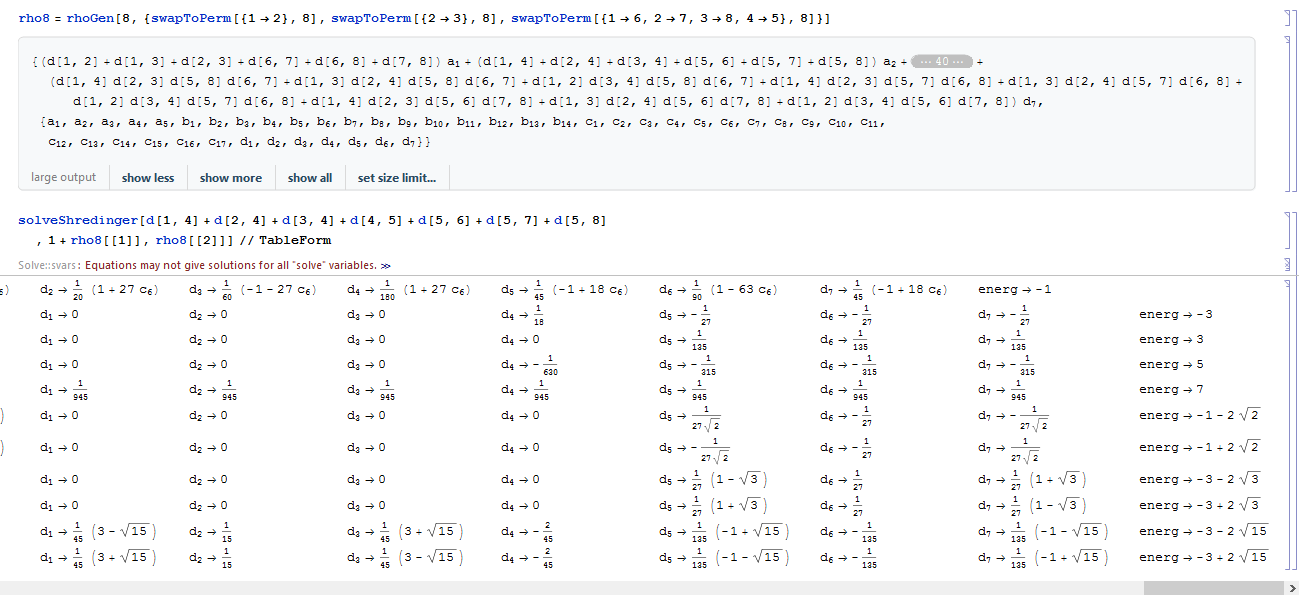
\includegraphics[width=1\linewidth]{result.png}
}
%----------------------------------------------------------------------------------------
%	LITERATURE
%----------------------------------------------------------------------------------------

\headerbox{References}{name=references,column=0,below=varpr,span=2}{
{\small
\begin{multicols}{2}

\renewcommand{\section}[2]{\vskip 0.05em} % Get rid of the default "References" section title
%\nocite{*} % Insert publications even if they are not cited in the poster
%\small{ % Reduce the font size in this block
\bibliographystyle{abbrv}
%unsrt
%
%\bibliography{C:/D/Work/QM/Bibs/1D,C:/D/Work/QM/Bibs/He} % Use sample.bib as the bibliography file
\bibliography{}
%}
\end{multicols}
}
}

\end{poster}

\end{document}

